\newpage

\section{Einfluss der Auger-Rekombination auf die IQE}
%
\begin{figure}[h!]
    \centering
    \begin{minipage}[t]{0.5\linewidth}
        \centering
        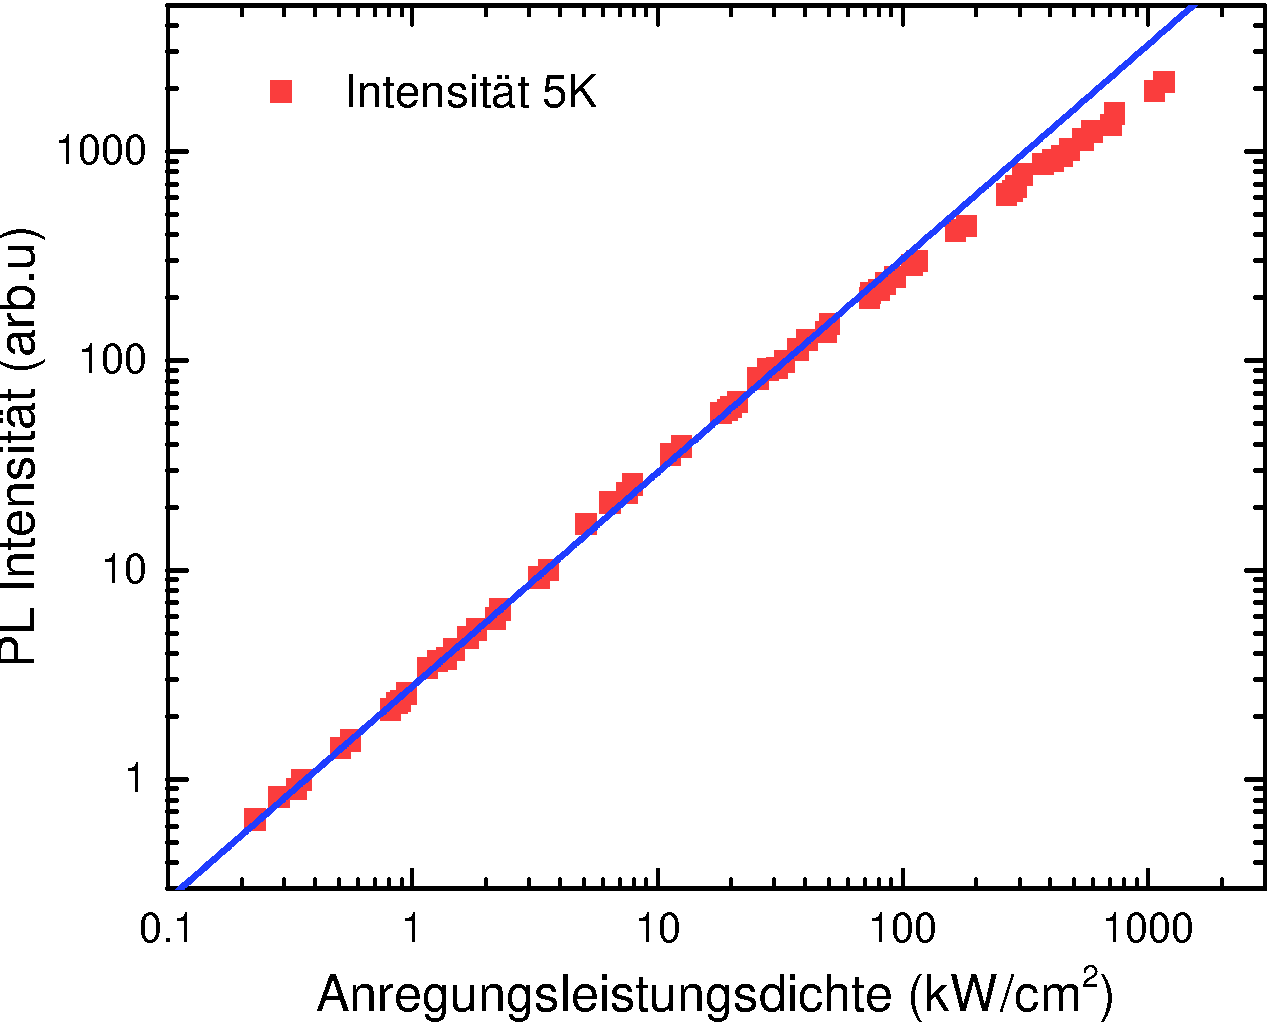
\includegraphics[width=\linewidth]{Bilder/AugerBei5K.pdf}
        \caption{}
        \label{fig:auger5k}
    \end{minipage}% <- sonst wird hier ein Leerzeichen eingefügt
\end{figure}
\raggedright
Das bisher benutzte Modell zur Bestimmung der PL-IQE ging davon aus, dass bei Tieftemperatur keine Auger-Rekombination (Gleichung) vorkommt, aber wie in Abb. [\ref{fig:auger5k}] deutlich zu erkennen, nimmt der Verlauf der PL-Intensität in doppeltlogarithmischer Darstellung gegenüber der Anregungsleistungsdichte die direkt proportional zur Ladungsträgerdichte ist, imBereich höherer Anregungsleistungen (entsprechend höheren Ladungsträgerdichten) deutlich ab und weist keinen linearen Verlauf mehr auf, den er aber durch eine allein quadratische Abhängigkeit (in doppeltlogarithmischer Darstellung linear) haben sollte. Dies zeigt,
dass die IQE nicht, wie bisher angenommen, immer bei 100 Prozent liegen sondern Anregungsleistungsdichte abhängig ist. Um dies zu berücksichtigen, wird nun die IQE bei 5K definiert als:
\begin{equation}
    IQE(5K) = Norm
\end{equation}
Die integrierte PL-Intensität wird durch die Anregungsleistungsdichte dividiert und auf das Maxmimum normiert, das bei der geringsten Anregungsleistungsdichte liegen sollte, so dass das Maximum der IQE bei $5K$ liegt. 

%
